\documentclass{article}

\usepackage[T1]{fontenc}
\usepackage{graphicx}
\usepackage{pict2e}
\usepackage{xcolor}
\usepackage{amsmath}
\usepackage[rflt]{floatflt}
\usepackage{graphicx,subfigure,epic,eepic}
\usepackage[most]{tcolorbox}
\usepackage{float}
\usepackage{caption}
\usepackage{fullpage}
\usepackage{hyperref}
\usepackage{fancyhdr}
\pagestyle{fancy}
\lhead{}
\rhead{}
\cfoot{}
\usepackage[top=5mm,includehead,headheight=45pt,
             left=1.5cm,bottom=2cm,right=1.5cm,headsep=0.3cm]{geometry} 

%inkscapestuff
\usepackage{import}
\usepackage{pdfpages}
\usepackage{transparent}
\usepackage{xcolor}

\newcommand{\incfig}[2][1]{%
    \def\svgwidth{#1\columnwidth}
    \import{./figures/}{#2.pdf_tex}
}

\pdfsuppresswarningpagegroup=1





\title{Three State Formalism}
\author{Vaibhav}

\begin{document}
\maketitle
\section{Boolean Formalism}
We have the following rules in boolean formalism for updating a node during simulations

\begin{itemize}

	\item $ S_j = 1 $ if    $  \sum_{ i } ^ { } adj[i][j] * S_i> 0 $ 

	\item $ S_j = -1 $ if    $  \sum_{ i } ^ { } adj[i][j] * S_i< 0 $

	\item In the case where the above sum is 0 we let the node have whatever state it had before and be somewhat `unregulated'

		\begin{figure}[H] \centering 
		
			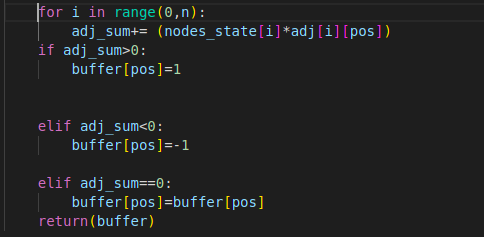
\includegraphics[scale=0.5]{img/boolean_formalism.png}
			\caption{Boolean Formalism}
		\end{figure}

		\begin{figure}[H]
		\centering
		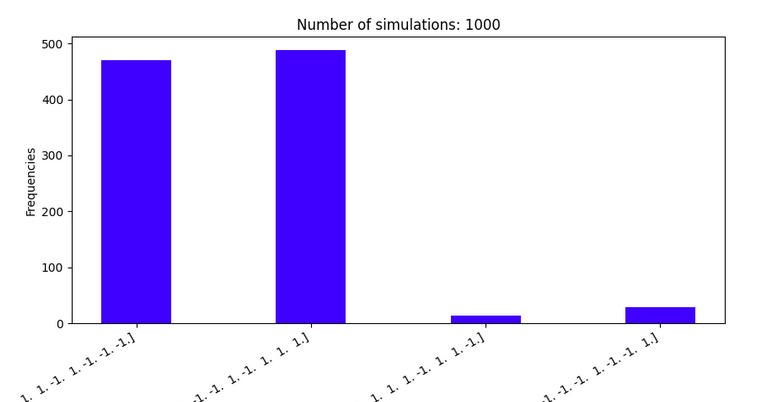
\includegraphics[scale=0.4]{img/emtracipe.png}
		\caption{EMT Racipe Boolean SSF}
		\end{figure}


		\begin{figure}[H]\centering
			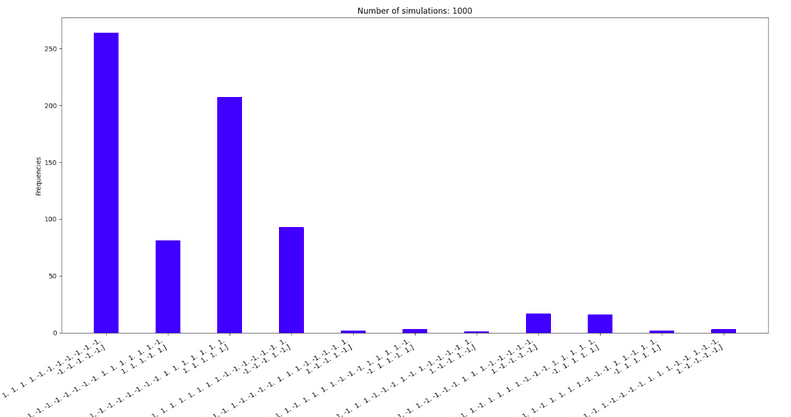
\includegraphics[scale=0.4]{img/emtracipe2boolssf.png}
			\caption{EMT Racipe 2 Boolean SSF}
		\end{figure}


\begin{figure}[H]
\centering 


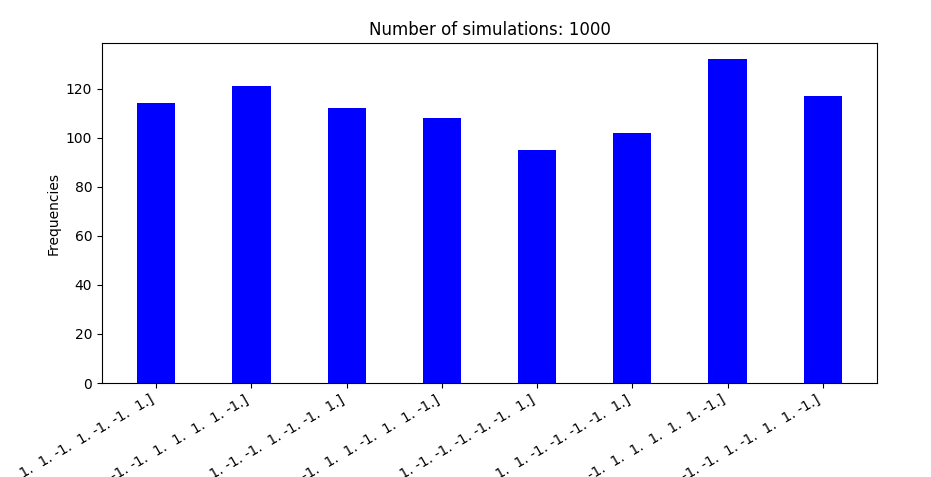
\includegraphics[scale=0.4]{img/melanomabooleanssf.png}
\caption{Melanoma Network Boolean SSF}
\end{figure}




\end{itemize}

\section{Three State Formalism}

Here we do not allow the unregulated nodes to affect other nodes. Therefore, 

\begin{itemize}

 	\item $ S_j = 1 $ if    $  \sum_{ i } ^ { } adj[i][j] * S_i> 0 $ 

	\item $ S_j = -1 $ if    $  \sum_{ i } ^ { } adj[i][j] * S_i< 0 $

	\item In the case where the above sum is 0 we introduce a third inactive state 0, incapable of any forward regulation. 
		
		\begin{figure}\centering
		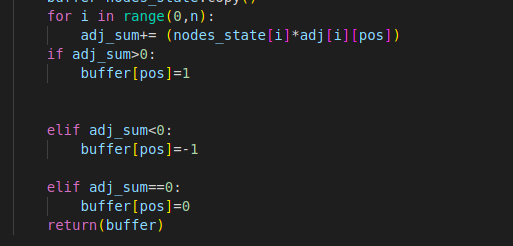
\includegraphics[scale=0.4]{img/terenary_formalism.png}
		\caption{Terenary Formalism}
		\end{figure}
\end{itemize}

Biologically it might mean that genes with basal production rates can't affect other genes

Upon simulating all the networks with three state formalism the following frequency distribution of states was obtained 



\begin{figure}[H]
	\centering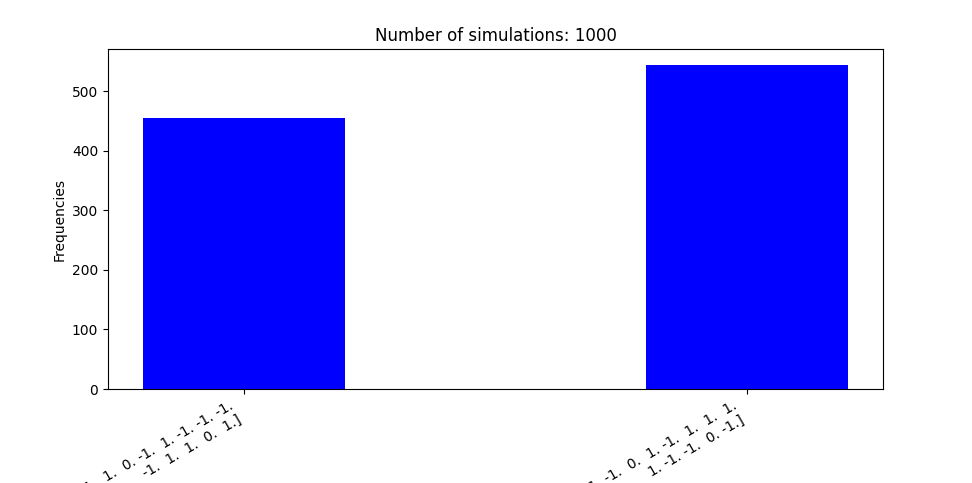
\includegraphics[scale=0.4]{img/emtracipe2ternaryssf.png}
	\caption{EMT Racipe 2 network simulated via terenary formalism}
\end{figure}
In the above figure, the two steady states have two nodes off which is different from the most frequent steady states obtained from boolean formalism 

\begin{figure}[H]\centering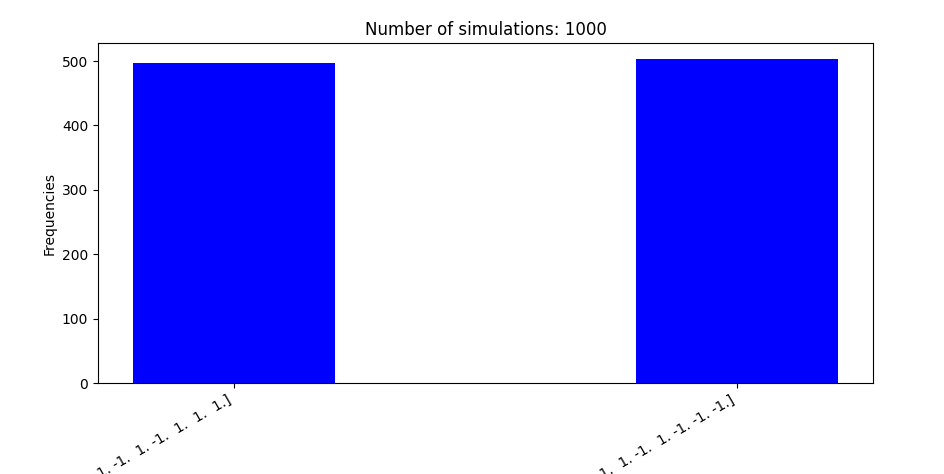
\includegraphics[scale=0.4]{img/emtracipeterenary.png}
	\caption{emt racipe terenary formalism}


\end{figure}


\begin{figure}[H]\centering
	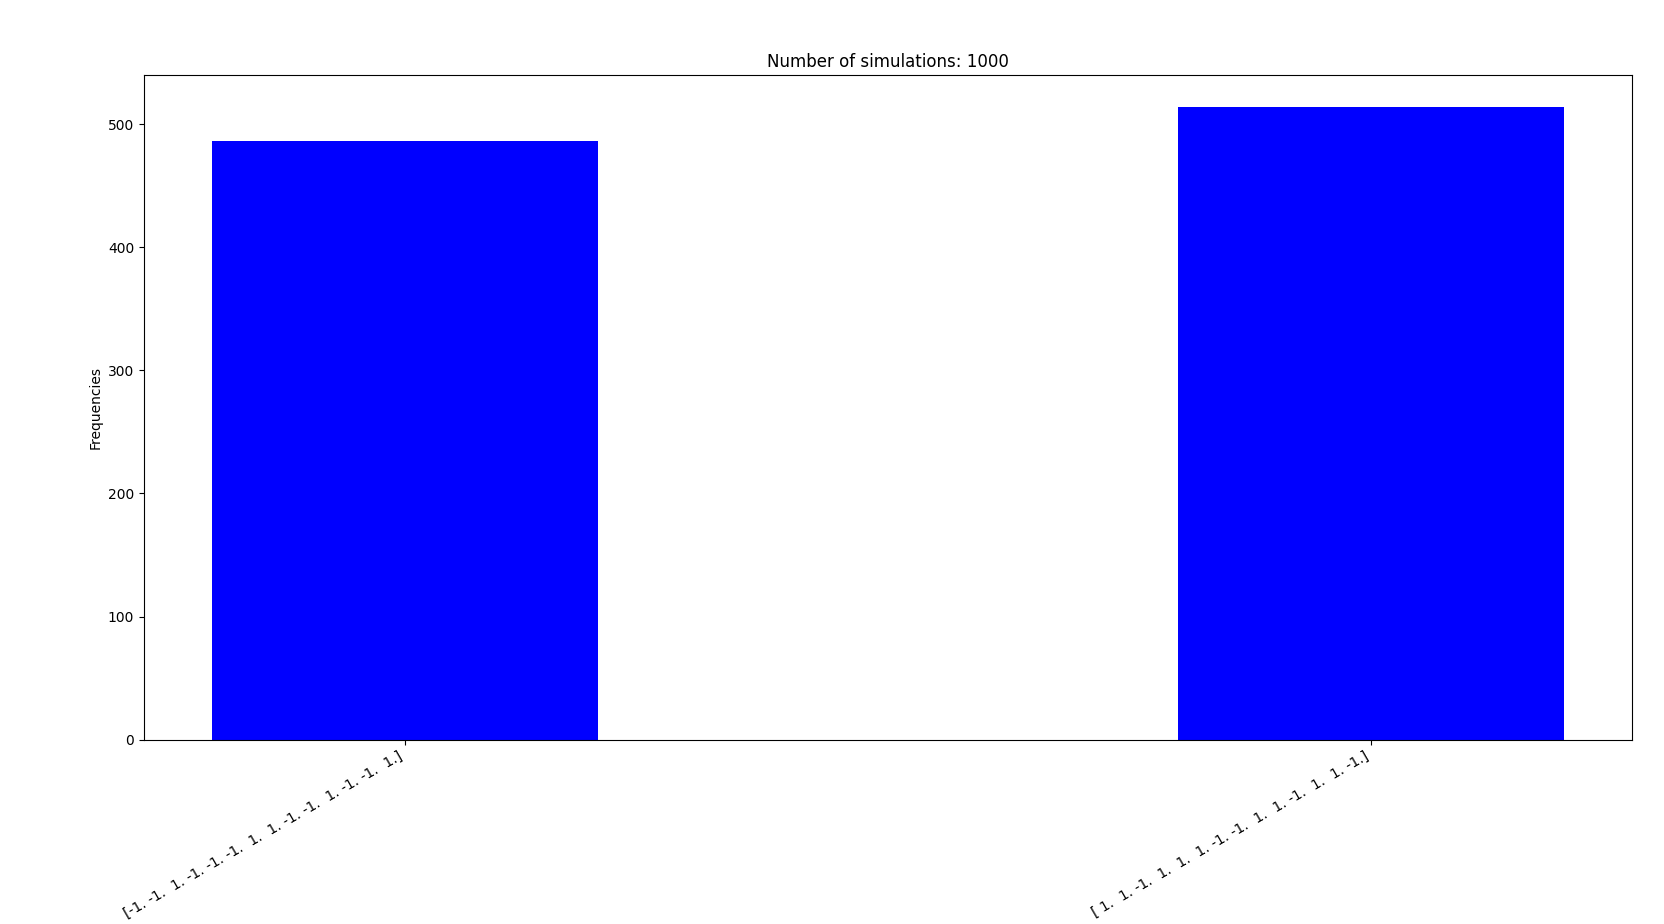
\includegraphics[scale=0.2]{img/melanomaterenarysim.png}
	\caption{Melanoma Network terenary }
\end{figure}





Upon inspecting all the hybrid states of emt racipe and emt racipe 2 network, it was found out that they all have at least one `loose/unregulated ' node 

Terenary formalism takes out the effect of the loose node and it is seen that most hybrid states obtained via boolean formalism, when simulated via terenary formalism fall into either of the two states obtained hence indicating that hybrid states are there because of the  `loose' nodes.  
\end{document}

